\documentclass[UTF8,a4paper,11pt,fontset=fandol]{ctexart}
\usepackage[margin=21mm]{geometry}
\usepackage{xurl,tikz}
\usetikzlibrary{arrows.meta}
\usepackage{booktabs,tabularx,array,xcolor,fancyhdr,hyperref,amsmath}
\definecolor{navy}{HTML}{183451}
\definecolor{teal}{HTML}{126B68}
\hypersetup{colorlinks=true,linkcolor=teal,urlcolor=teal,pdftitle={Ripple 弱网带宽优化},pdfauthor={袁靖淳}}
\ctexset{section={format=\Large\bfseries\color{navy}},subsection={format=\large\bfseries\color{teal}}}
\pagestyle{fancy}\fancyhf{}\lhead{\small 面向对象程序设计课程大作业}\rhead{\small Ripple}\cfoot{\thepage}\setlength{\headheight}{15pt}
\setlength{\parindent}{2em}\setlength{\parskip}{3pt}\renewcommand{\arraystretch}{1.2}
\newcolumntype{Y}{>{\raggedright\arraybackslash}X}
\newcommand{\code}[1]{\nolinkurl{#1}}
\begin{document}
{\color{navy}\huge\bfseries Ripple 弱网带宽优化\par}
\vspace{5mm}

\section{项目代码分析}
Ripple 是一个发布订阅系统。发布者向服务端写入键值，订阅者按应用名和键接收更新。
\subsection{客户端与服务端依赖哪些代码}
利用 IntelliJ IDEA 的依赖矩阵查看 Ripple 项目的包结构（图~\ref{fig:idea-dsm}）。客户端与服务端之间的交叉区域是空的，说明两者没有直接的代码依赖。两端共同使用的消息类型、编解码器等被放在 \code{ripple-common} 模块中；客户端和服务端的 Maven 配置也都依赖这个模块，而不依赖对方。

\begin{figure}[htbp]
\centering
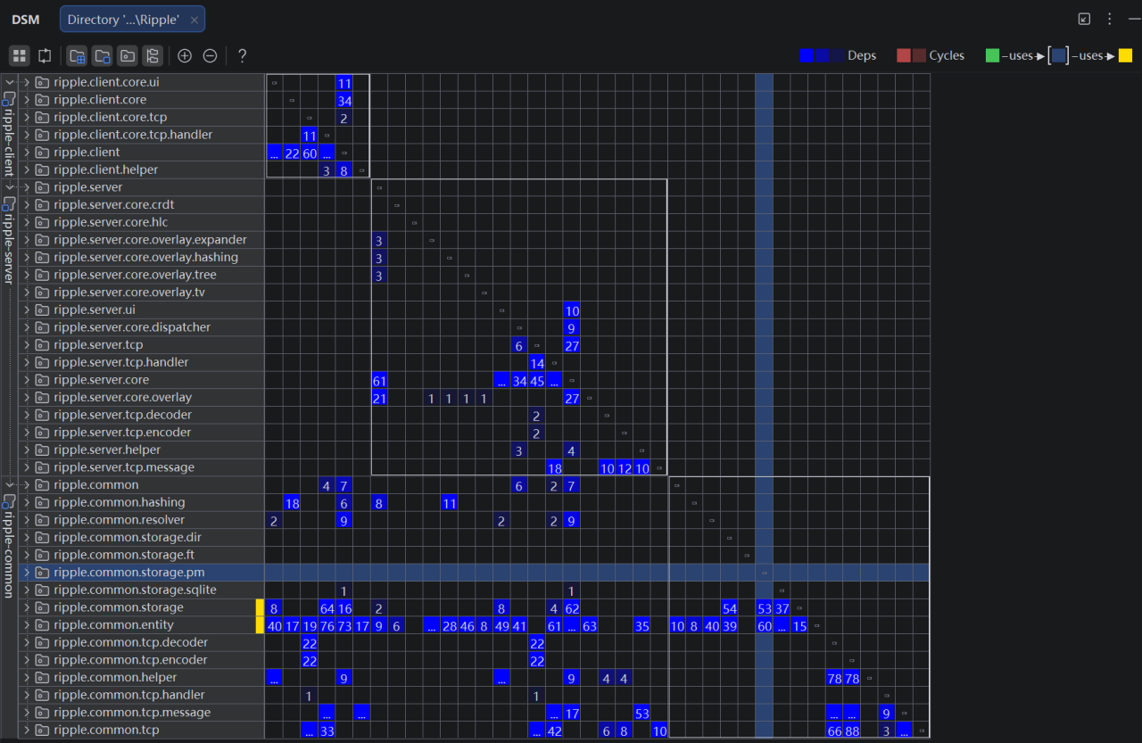
\includegraphics[width=\linewidth]{images/ripple-idea-dsm.png}
\caption{IntelliJ IDEA 中的 Ripple 包依赖矩阵}
\label{fig:idea-dsm}
\end{figure}

服务端调整副本转发策略，不需要改客户端；同步帧的类型和字段格式却必须两端一致，因此由 \code{ripple-common} 维护。这让两端可以分别修改业务逻辑，在协议变化时统一通信双方的编码格式。

\newpage
\subsection{一次 PUT 如何到达订阅端}
\begin{figure}[htbp]
\centering
\begin{tikzpicture}[x=1cm,y=1cm,font=\footnotesize,arr/.style={-{Stealth[length=1.6mm]},draw=navy},wire/.style={arr,draw=teal,line width=.8pt},lab/.style={above,fill=white,inner sep=1pt,font=\scriptsize}]
\foreach \l/\r/\t in {-.70/.70/发布者,.79/2.70/发送端,2.80/10.65/服务端,10.75/15.25/接收端}{\fill[navy!8] (\l,.8) rectangle (\r,1.35);\node[text=navy] at ({(\l+\r)/2},1.08){\t};}
\foreach \x/\name in {0/用户,1.74/RippleClient,3.90/\shortstack{PutRequest\\Handler},5.94/Node,7.80/Storage,9.64/\shortstack{Client\\Dispatcher},11.97/\shortstack{SyncRequest\\Handler},14.35/Storage}{\node[align=center,font=\scriptsize] at (\x,.41){\name};\draw[dashed,gray!65] (\x,.02)--(\x,-5.35);}
\draw[arr] (0,-.5)--node[lab]{put(...)}(1.74,-.5);
\draw[wire] (1.74,-1.1)--node[lab]{PUT\_REQUEST}(3.90,-1.1);
\draw[arr] (3.90,-1.7)--node[lab]{put(...)}(5.94,-1.7);
\draw[arr] (5.94,-2.05)--++(.48,0)--++(0,-.32)--(5.94,-2.37);\node[anchor=west,fill=white,font=\scriptsize] at (6.44,-2.19){创建 UpdateMessage};
\draw[arr] (5.94,-2.92)--node[lab]{保存更新}(7.8,-2.92);
\draw[arr] (5.94,-3.52)--node[lab]{按订阅关系通知}(9.64,-3.52);
\draw[wire] (9.64,-4.12)--node[lab]{SYNC\_REQUEST}(11.97,-4.12);
\draw[arr] (11.97,-4.48)--++(.39,0)--++(0,-.29)--(11.97,-4.77);\node[anchor=east,fill=white,font=\scriptsize] at (11.90,-4.64){还原更新消息};
\draw[arr] (11.97,-5.23)--node[lab]{写入本地存储}(14.35,-5.23);
\end{tikzpicture}
\caption{一次普通更新的对象时序（单服务端、单订阅者）}
\end{figure}

发布者调用 \code{RippleClient.put} 后，消息先以 PUT 请求到达服务端。\code{PutRequestHandler} 将请求交给 \code{Node}，由它生成带业务 UUID 的更新、写入存储，再通过 \code{ClientDispatcher} 通知订阅了同一应用名和键的客户端。第二段传输使用同步请求：接收端由 \code{SyncRequestHandler} 还原更新并写入自己的存储，到这里才算订阅交付。发布者收到 PUT 成功响应和订阅者收到更新，是这条路径上的两个不同时刻。

\newpage
\section{网络带宽优化的背景}
现有消息引擎只能在网络良好的地区使用，对于网络带宽差的地方，需要进行格外的优化以降低所传输数据包的大小以及延迟。


\subsection{限制带库复现积压现象}
实验使用一个服务端、一个发布者和一个订阅者。订阅下行限为 1 KiB/s，发布者每秒发送一条 2 KiB 的消息，持续 60 秒。
仅正文的发送速率就是下行容量的两倍。测试会记录60s消息时还有多少条消息积压，以及最终消息被完全接收的时间。

\begin{center}\begin{tabular}{lrrr}\toprule
下行条件 & 60 秒时已处理 & 停发后收齐（s） & 内容正确\\\midrule
仅限速 & 24 & 79.980 & 60/60\\
限速加 2 秒传播延时 & 23 & 81.764 & 60/60\\
限速加 50\% 随机包丢失 & 4 & 1141.725 & 60/60\\\bottomrule
\end{tabular}\end{center}

仅限速时，停发后仍需约 80 秒才能收齐。加入丢包后，消息最终都收到，但由于TCP协议的指数重试造成
了积压的增加。

\section{具体优化措施}
\begin{enumerate}
\item \textbf{减少消息协议的长度。} 缩短每帧都要发送的标识和类型字段，不改变消息内容。
\item \textbf{添加压缩器与解压缩器。} 发送端压缩普通更新的正文，接收端将其还原。
\end{enumerate}

\newpage
\subsection{减少消息协议的长度：字段对照与理论收益}
以普通更新同步请求（\code{SYNC_REQUEST}，操作为 \code{update}）为例。下表按写入顺序比较原版与紧凑协议；两组使用相同的应用名、键和正文，均关闭正文压缩。

\begin{center}\small
\begin{tabularx}{\linewidth}{@{}lYYr@{}}\toprule
协议字段 & 原有表示 & 修改后表示 & 节省（B）\\\midrule
帧长度、消息类型 & 4 B 长度 + 1 B 类型 & 共用 4 B 帧头 & 1\\
请求 UUID & 4 B 长度 + 36 B 文本 & 两个 8 B 整数 & 24\\
业务消息 UUID & 4 B 长度 + 36 B 文本 & 两个 8 B 整数 & 24\\
操作类型 & 4 B 长度 + 6 B 的 \code{update} & 1 B 操作码 & 9\\
应用名、键、正文 & 各为 4 B 长度 + UTF-8 内容 & 不变 & 0\\
最后更新时间 & 8 B 时间戳 & 不变 & 0\\
最后更新节点、来源节点 & 两个 4 B 节点 ID & 不变 & 0\\\midrule
每条普通更新同步请求 & & & \textbf{58}\\\bottomrule
\end{tabularx}\end{center}

\textbf{每条省多少？} 两个 UUID 省 48 B，操作类型省 9 B，打包帧头再省 1 B，合计 \textbf{58 B}。例如，原先 147 B 的同步帧，启用紧凑 UUID 和操作码后为 90 B，再启用打包帧头后为 89 B。对相同类型的更新，正文长短不影响这 58 B；其他消息的字段组合不同，不能直接套用这个数。

\subsubsection{UUID：从字符表示改为二进制表示}
例如 \code{550e8400-e29b-41d4-a716-446655440000}，原版 UUID 由 32 个十六进制字符和 4 个连字符组成。每个字符用 UTF-8 编码占 1 B，因此字符串占 36 B；再加上字符串编码写入的 4 B 长度，共占 40 B。

UUID 的有效信息只有 $32\times4=128$ bit，即 16 B。修改后直接发送这 128 位，不再发送连字符，也不再写长度。每个 UUID 因而从 40 B 降到 16 B，\textbf{节省 24 B，减少 60\%}。普通同步请求包含请求 UUID 和业务消息 UUID，合计省下 48 B；UUID 的值和唯一标识用途保持不变。

\subsubsection{修改了哪些类和方法}
\code{TypeHelper} 是 UUID 编解码的公共工具类。修改这个入口后，调用它的请求和响应可以共用同一套二进制表示，无需在各个处理器里重复实现。
\begin{itemize}\setlength{\itemsep}{2pt}
\item \code{writeUuid(UUID, ByteBuf)}：原来调用 \code{writeString(value.toString(), ...)} 写字符串；现在通过 \code{getMostSignificantBits()} 和 \code{getLeastSignificantBits()} 取出高、低各 64 位，再用两次 \code{writeLong()} 写入，共 16 B。
\item \code{readUuid(ByteBuf)}：原来先读字符串，再用 \code{UUID.fromString()} 解析；现在用两次 \code{readLong()} 取回高、低位，再通过 \code{new UUID(...)} 还原对象。
\item 新增 \code{isCompactWire()}：读取 JVM 参数 \code{ripple.wire.compact}。两端启用 \code{-Dripple.wire.compact=true} 时使用紧凑格式；未启用时仍走原来的字符串编解码路径。
\end{itemize}

\code{SyncRequestEncoder.operationCode()} 将普通更新、删除、增量更新映射为 1、2、3；\code{SyncRequestDecoder.operationType()} 将操作码还原为原有字符串常量。\code{PackedFrame} 定义组合帧头，\code{MessageEncoder.encode()} 写入长度和类型，\code{MessageDecoder.decode()} 提取类型，\code{PackedFrameDecoder.decode()} 按长度拆帧。这样，字段的缩短集中在编解码代码中，业务处理器仍接收原来的 UUID 和操作类型。

\subsection{添加压缩器与解压缩器}

本次采用 DEFLATE 无损压缩：先用 LZ77 查找重复字节串，用“向前的距离和长度”代替再次写入相同内容，再用 Huffman 编码缩短字面量与匹配信息的表示。英文中的重复单词和句式因而有机会用更少的字节存储，解压后可逐字节还原正文。

代码通过 JDK 提供的压缩器实现，选择 \code{BEST_SPEED}，优先缩短压缩处理时间；使用 raw DEFLATE 数据流，不附带 zlib 包装头和校验尾。原文长度和压缩长度由 Ripple 协议字段记录，接收端据此校验解压结果。

\code{PayloadCodec} 在发送端用 \code{Deflater} 压缩正文，在接收端用 \code{Inflater} 还原。设原文为 $N$ 字节、压缩后为 $C$ 字节：原格式占 $4+N$ B，压缩格式要同时记录压缩长度和原文长度，占 $8+C$ B。因此，普通更新正文达到 512 B 才尝试压缩，且只有 $8+C<4+N$ 时才发送压缩结果；否则仍发原文。

接收端按帧头标志选择解码方式，恢复的仍是原来的业务字符串。与第一项固定节省的 58 B 不同，第二项的额外收益取决于正文内容，下一节用整份文本测量。

\newpage
\section{优化后的对照实验}
\subsection{字段紧凑化后的实测提升}
之前的测试单独比较了 UUID 二进制表示和单字节操作码。正文保持不变，不启用正文压缩。编码测试对每组 1,000 条消息逐条解码核对；网络测试采用三台服务端、一名订阅者，订阅下行限为 512 kbit/s，按每秒 50 条的目标速率发送 2 秒，再等待 3 秒。以下选取 32 B 小消息的结果。

\begin{center}\small\begin{tabular}{lrrr}\toprule
比较指标 & 优化前 & 字段紧凑化后 & 减少比例\\\midrule
单条同步应用帧（B） & 173 & 116 & 32.95\%\\
下行抓包总字节（B） & 23,793 & 18,150 & 23.72\%\\
平均每条下行抓包字节（B） & 240.33 & 183.33 & 23.72\%\\
正式发送／接收条数 & 99／99 & 99／99 & ---\\\bottomrule
\end{tabular}\end{center}

单条同步帧恰好少了 57 B，与两个 UUID 节省 48 B、操作类型节省 9 B 的计算一致。该次实测尚未打包帧头，因此比前面完整方案的 58 B 少 1 B。实际下行抓包包含 TCP/IP 和链路头等开销，降幅为 23.72\%；两组均完整收到 99 条消息，内容异常为零。对正文只有 32 B 的更新，缩短固定字段就能明显降低下行流量。

数据来自归档的 \code{codec-ledger.json} 和 \code{results.csv}（\code{docs/experiments/bandwidth_20261022}）。本组先验证固定字段的收益，下一组再测压缩正文能额外省下多少字节。

\subsection{比较压缩开关性能差距}
三档都发送同一份 103,613 B 的《小王子》英文纯文本。按 1、10、100 KiB 的正文上限顺序切分，切点避开 UTF-8 字符中间，末块不补齐。两组都启用紧凑编码和打包帧头，只切换正文压缩。解码后将各块拼回，并与原文件逐字节核对。

大小是发送整份文本的应用帧总字节数。预编码后的帧通过已连接、未限速的本机 TCP 回环发送，从发送端写入帧流到收到接收端的收齐确认为止。计时不含建连、压缩或编解码。每档预热 20 轮后取 31 轮的中位数，两组轮换先后顺序。

\begin{center}\small\begin{tabular}{lrrrrrr}\toprule
正文上限 & 消息数 & 关压缩（B） & 开压缩（B） & 降幅 & 关（ms） & 开（ms）\\\midrule
1 KiB & 102 & 111,161 & 59,617 & 46.37\% & 0.509 & 0.288\\
10 KiB & 11 & 104,427 & 44,138 & 57.73\% & 0.555 & 0.318\\
100 KiB & 2 & 103,761 & 40,460 & 61.01\% & 0.478 & 0.225\\
\bottomrule
\end{tabular}\end{center}

在 100 KiB 档，压缩把总帧大小从 103,761 B 降到 40,460 B，TCP 传输耗时中位数从 0.478 ms 降到 0.225 ms。1 KiB 档同样省字节，但需要 102 条消息；对这份文本，更多的小块意味着更多帧开销，也让压缩器能利用的上下文更短。

\newpage
\section{结论与复现}
固定字段优化和正文压缩解决的是两类问题。前者思路是让每条消息的额外协议层尽可能精简到按比特来表示协议字段，为示例同步请求固定节省 58 B，对短消息尤其直接；后者取决于正文和分块，在这次全文实验中又减少了 46.37\% 至 61.01\% 的应用帧字节。

由于压缩器会根据具体压缩情况来分派是否压缩，所以在带宽方面这项改动只有收益，但是可能会给cpu造成额外压力，可以根据具体情况调整是否开启。

\subsection{复现与材料}
在 \code{Ripple-versions} 源码目录运行下列命令。全仓测试共 18 项通过；专项测试将每档的帧大小和 TCP 传输耗时输出到以 \code{WIRE\_RESULT} 开头的行。
\begin{verbatim}
mvn test
mvn -pl ripple-common -Dtest=CompactWireTest test
\end{verbatim}
\begin{itemize}
\item \code{FrameCompression.zh-cn.md}：样本来源、排版处理及实验步骤。
\item \code{FrameCompression-results.csv}：全文分块实验的原始测量数据。
\item \code{ripple-slow-link-results-20261022.md} 与 \code{ripple-bandwidth-verified-20261022.md}：原版积压实验和历史下行抓包。
\end{itemize}
\end{document}
